\newcommand{\EvaluationTitle}{Evaluation}
\begin{frame}
    \frametitle{\EvaluationTitle}
    \centering
    \begin{minipage}{1\textwidth}
        \begin{itemize}%[<+->]
            \item Setup
            \begin{itemize}
                \item Graph file simulator
            \end{itemize}
            \item Test
            \item Validation
            \begin{itemize}
                \item Latency
                \item Outgoing packet validation
                \item Internet Protocol Suite
                compliancy as per RFC
                1122
            \end{itemize}
        \end{itemize}
    \end{minipage}
\end{frame}

\begin{frame}[fragile]
    \frametitle{\EvaluationTitle}
    \framesubtitle{Setup}
    Graph file simulation\\
    \begin{itemize}%[<+->]
        \item Full input - output
        \item Does not take latency between packets into account
        \item Simplifies test cases
    \end{itemize}
\end{frame}


\begin{frame}[fragile]
    \frametitle{\EvaluationTitle}
    \framesubtitle{Setup}
    \begin{columns}
        \begin{column}{0.45\textwidth}
            \centering
            Graph simulation node types\\
            \begin{figure}
                \centering
                \begin{minipage}{0.33\textwidth}
                    \centering
                    \includegraphics[scale=0.45]{evaluation/dot_files/datain.eps}
                    Data In
                    \label{fig:packet_graph_datain}
                \end{minipage}%
                \begin{minipage}{0.33\textwidth}
                    \centering
                    
\includegraphics[scale=0.45]{evaluation/dot_files/send.eps}
                    Send
                    \label{fig:packet_graph_send}
                \end{minipage}%
                \begin{minipage}{0.33\textwidth}
                    \centering
                    \includegraphics[scale=0.45]{evaluation/dot_files/command.eps}
                    Command
                    \label{fig:packet_graph_command}
                \end{minipage}%
                \\
                \begin{minipage}{0.33\textwidth}
                    \centering
                    \includegraphics[scale=0.45]{evaluation/dot_files/dataout.eps}
                    Data Out
                    \label{fig:packet_graph_dataout}
                \end{minipage}%
                \begin{minipage}{0.33\textwidth}
                    \centering
                    
\includegraphics[scale=0.45]{evaluation/dot_files/receive.eps}
                    Receive
                    \label{fig:packet_graph_receive}
                \end{minipage}%
                \begin{minipage}{0.33\textwidth}
                    \centering
                    \includegraphics[scale=0.45]{evaluation/dot_files/wait.eps}
                    Wait
                    \label{fig:packet_graph_wait}
                \end{minipage}%
            \end{figure}%
        \end{column}
        \begin{column}{0.55\textwidth}
            {\renewcommand{\arraystretch}{1.5}
            \begin{table}
                \begin{center}
                    \begin{tabular}{lc}
                        State and Color &Description\\ \hline \hline
                        \statecolorboxtext{graph_waiting}{Waiting} &
                        \makecell{Vertex is not in use.}\\ \hline

                        \statecolorboxtext{graph_isready}{Ready} &
                        \makecell{Vertex Is ready\\ for activation.}\\ \hline

                        \statecolorboxtext{graph_active}{Active} &
                        \makecell{Vertex is active.\\ Simulator is\\ gathering data.}\\ \hline

                        \statecolorboxtext{graph_inactive}{Inactive} &
                        \makecell{Vertex is inactive.\\Simulator is not\\ gathering data.}\\ \hline

                        \statecolorboxtext{graph_done}{Done} &
                        \makecell{Vertex is done\\ and validated.}
                    \end{tabular}
                \end{center}
            \end{table}
            }
        \end{column}
    \end{columns}
\end{frame}

\begin{frame}[fragile]
    %\frametitle{\EvaluationTitle}
    %\framesubtitle{Test}
    \begin{columns}
        \begin{column}{0.50\textwidth}
            \begin{figure}
            \centering
                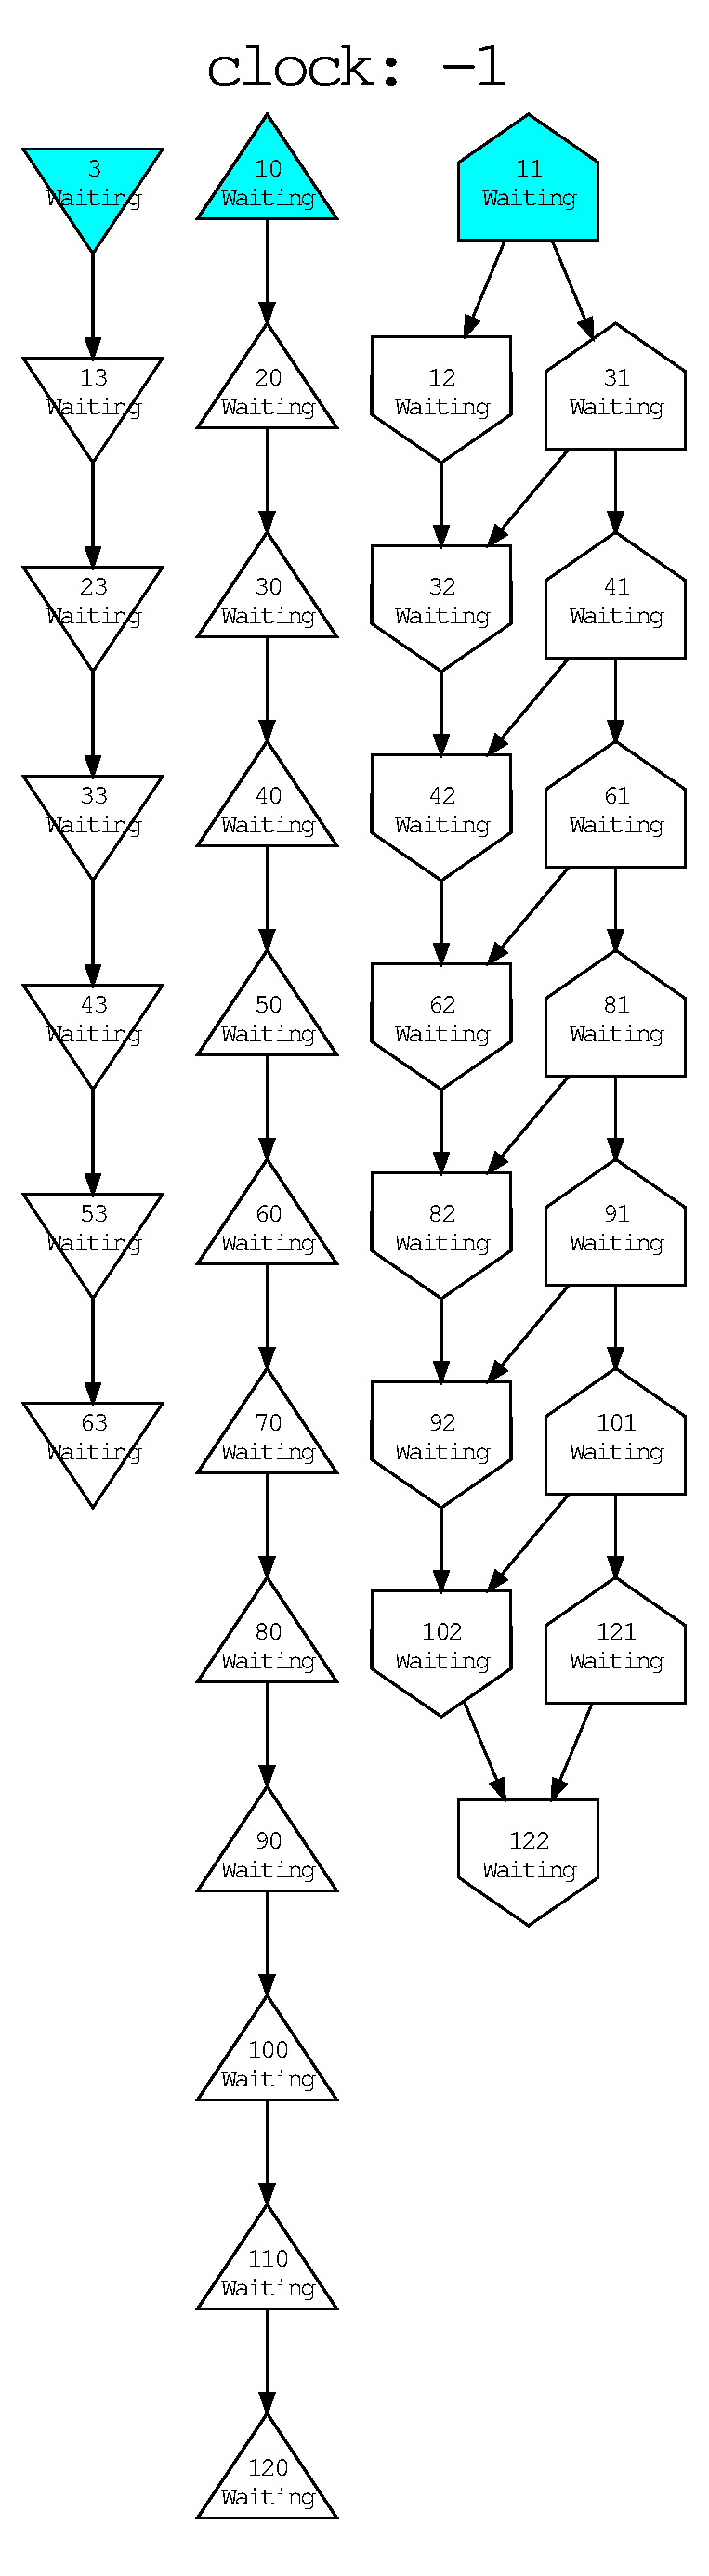
\includegraphics[scale=0.20]{evaluation/dot_files/example_graph_initial.eps}
                \caption{The initial state of a simulation}
            \end{figure}
        \end{column}
        \begin{column}{0.50\textwidth}
            \begin{figure}
                \centering
                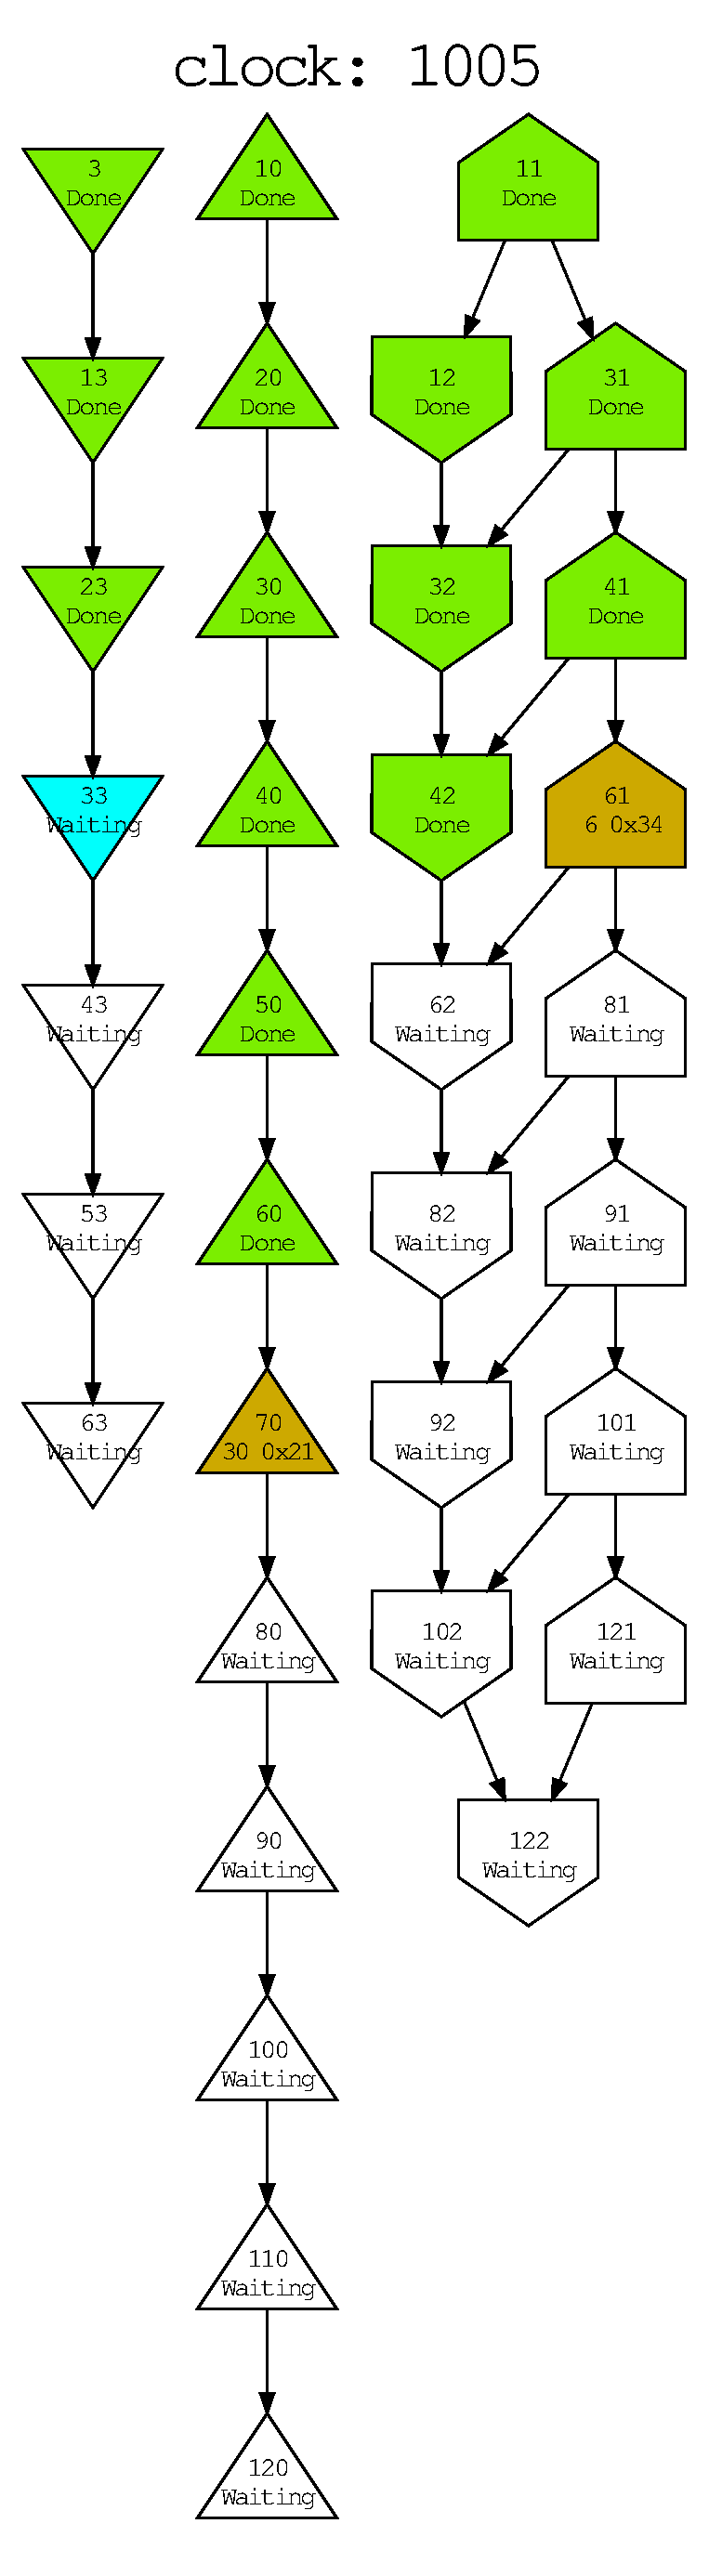
\includegraphics[scale=0.20]{evaluation/dot_files/example_graph_running.eps}
                \caption{The state after 1005 clocks}
            \end{figure}
        \end{column}
    \end{columns}
\end{frame}